\section{Results}
\subsection{Model Performance}\label{subsec:model-performance}
Overall, the models developed as part of the intelligence hierarchy performed fairly well.
\autoref{fig:apple-tree-mode-training-curve} demonstrates a learning curve for one of the first-layer apple-in-view models.

\begin{figure}[!htb]
    \centering
    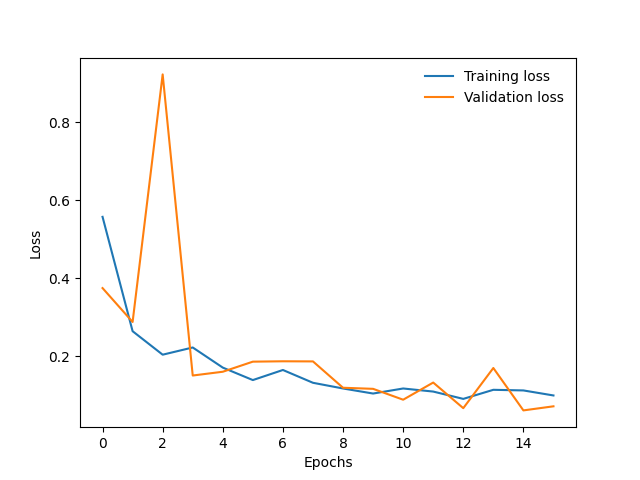
\includegraphics[width=\columnwidth,keepaspectratio]
    {./figures/mobile_model_apple_trees_16its_2022-11-15_training_curve}
    \caption{
        Learning curve for a apple-in-view CNN.
        The model is a retrained version of MobileNet~\cite{Sandler2018,PyTorchMobileNet}, which is a more light-weight while still very powerful CNN.
        Loss is in mean squared error.
    }
    \label{fig:apple-tree-mode-training-curve}
\end{figure}




\subsection{Robot Performance}\label{subsec:robot-performance}

